\documentclass[12pt,a4paper,twoside,titlepage]{article}
\usepackage[utf8]{inputenc}
\usepackage[english,german]{babel}
\usepackage{utopia}
\usepackage{makeidx}
\usepackage{graphicx}
\usepackage[onehalfspacing]{setspace}
\usepackage{fancyhdr}
\usepackage{lastpage}
\usepackage{hyperref}
\usepackage{textcomp}
\renewcommand{\sffamily}{phv}

\usepackage[margin=1in]{geometry}
\newcommand{\titleText}{Facharbeit zu \textbf{Die Verwandlung} von \textbf{Franz Kafka}}
\newcommand{\authorText}{Patrick Günthard}
\newcommand{\dateText}{\today}

\title{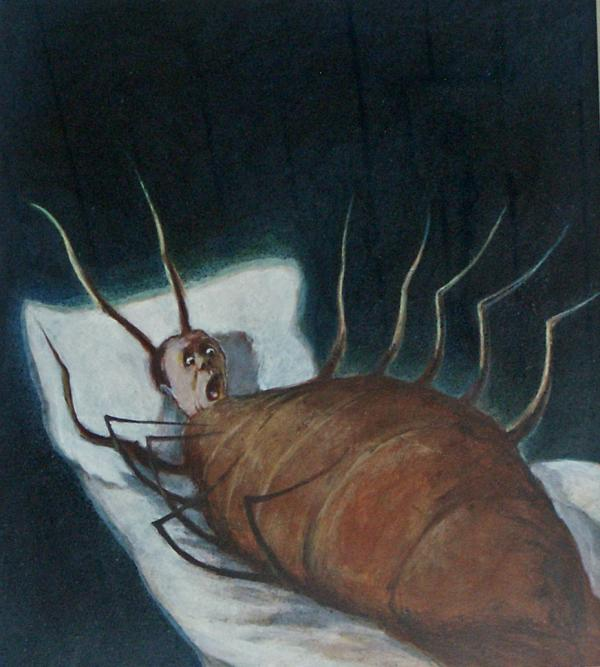
\includegraphics[width=7cm]{metamorphosis-kafka}\small\textit{\textcopyright The Quick Word\ref{qui14}}\huge\\\titleText}
\author{\authorText}
\date{\dateText}

\pagestyle{fancy}
\fancyhf{}

\fancyhead[EL]{\titleText}
\fancyhead[OR]{\authorText}
\cfoot{\thepage \space von \pageref{LastPage}}

%\renewcommand{\familydefault}{\sfdefault}
%\fontfamily{phv}\selectfont


\begin{document}
	\maketitle
	
	\tableofcontents
	
	\section{Einleitung}
	
	
	Das Buch \textit{Die Verwandlung} von \textit{Franz Kafka} ist teilweise sehr surrealistisch und arbeitet viel mit Symbolik. Die Geschichte lässt sich dadurch auf viele mögliche Szenarien herunter brechen und analysieren.
	
	Diese Arbeit fokussiert sich vor allem auf die Analyse der Interaktion der Charaktere und versucht die Entwicklung und auch die mögliche Degeneration von zwischenmenschlichen Beziehungen aufzuzeigen.
	
	Gerade die Entfremdung der Beziehungen, welche von unserer Umgebung erzwungen werden, sind ein Schwerpunkt dieser Arbeit.
	
	
	\subsection{Fragestellung}
	Die Fragestellung zur Arbeit lautet folgendermassen:
	\begin{itemize}
		\item Wie verändert sich die Beziehung von Gregor zu seinem Umfeld?
		\begin{itemize}
			\item Wie verändert sich die Beziehung zu seiner Schwester?
			\item Wie verändert sich die Beziehung zu seinen Eltern?
		\end{itemize}
	\end{itemize}
	
	Die Fragestellung ist aus dem Gedanken entstanden, wie diese Geschichte in einem realistischeren Beispiel ausgesehen hätte. Es findet eine starke Entfremdung des Protagonisten \textit{Gregor Samsa} statt. Im Buch wird diese sehr symbolisch dargestellt, indem er sich in ein Ungeziefer verwandelt welches niemand mehr sehen wollte. Auch kann er nicht mehr mit seiner Familie sprechen da ihn niemand mehr versteht. Wenn er zu sprechen versucht, gibt er nur unverständliche Laute von sich. Er hingegen versteht noch alles, was die Menschen um ihn sagen.
	
	\subsection{Zusammenfassung}
	
	\textit{Die Verwandlung} von \textit{Franz Kafka} handelt von einem Mann mit dem Namen \textit{Gregor Samsa}, welcher sich eines Tages über Nacht in ein Ungeziefer verwandelt. Sein Bewusstsein bleibt vollständig erhalten, jedoch ist es ihm nicht mehr möglich, mit der Aussenwelt zu kommunizieren. Auch wirkt sein neues Aussehen verstörend auf seine Familie.
	
	\textit{Gregors} Rolle vor seiner Verwandlung war eine sehr wichtige. Er war der einzige, der arbeiten ging und als reisender Händler den Unterhalt für die Familie verdiente. \footnote{\cite{verwandlung} Kap. 1, Abs. 4}
	
	Er bleibt in seinem Zimmer eingesperrt und wird von der Familie kaum noch beachtet. Anfangs versucht seine Schwester sich um ihn zu kümmern, jedoch ist sie gegen Ende die grösste Befürworterin das Ungeziefer in das sich \textit{Gregor} verwandelt hat zu töten.
	
	Seine Familie versucht ihn zu ignorieren und irgendwie auch das fehlende Einkommen \textit{Gregors} über die Runden zu kommen. Sie vermieten ein Zimmer des Hauses. Als die Untermieter das Ungeziefer das erste mal sehen, ziehen sie jedoch gleich wieder aus.
	
	\textit{Gregor} wurde von verschiedenen Personen mehrmals physisch angegriffen. Er trug mehrere Verletzungen davon welche auch nach mehreren Tagen noch nicht verheilt waren. Es ging ihm immer schlechter, bis er schlussendlich starb. Dir Familie war wieder glücklich und sieht sein Tod als eine \textit{Erlösung}
	
	\subsection{Motivation}
	
	In der Realität ist eine solche Entfremdung nicht unrealistisch, jedoch drückt sie sich viel langsamer und auf völlig anderen Ebenen aus. Die Art wie sich die Reaktionen der Mitmenschen ausdrückt unterscheidet sich natürlich auch sehr stark. In gewissen Fällen kann man jedoch die selben Muster erkennen und vor allem die Veränderung der Beziehungen zwischen den Personen passieren oft nach einem ähnlichen Prinzip. 
	
	Wie diese Entfremdung in der Realität aussieht wird in dieser Arbeit nicht beantwortet. Natürlich könnte man diese These mit wissenschaftlichen Methoden beweisen oder auch widerlegen. Da dies jedoch nicht der Aufgabenstellung entspricht und den Rahmen der Arbeit sprengen würde, wird diese These nicht behandelt. Daher dient diese Fragestellung eher als Motivation für diese Arbeit als dass sie ein wissenschaftlicher Teil davon wäre.
	
	
	
	\section{Veränderung der Beziehung zu seinem persönlichen Umfeld}
	Das Buch zeigt nur ein ganz kleiner Ausschnitt aus der Beziehung zwischen \textit{Gregor} und seiner Familie. Der grösste Teil findet vor der Handlung des Buches statt und über die Details kann nur spekuliert werden. Es gibt mehrere Punkte welche \textit{Gregor's} Leben vor seiner Handlung beschreiben, deren Erwähnung für die Analyse notwendig sind.
	
	So war \textit{Gregor} als reisender Händler tätig.\footnote{Ebd. Kap. 1, Abs. 4} Er mochte sein Beruf nicht, er dachte er bedeute zu viel Stress und Arbeit. \textit{,,Die Geschäftlichen Aufregungen''}, meint er, seien \textit{,,viel grösser, als im eigentlichen Geschäft.''} \footnote{Ebd. Kap. 1, Abs. 4}
	
	\textit{Gregor} lebt mit seinen Eltern und seiner Schwester zusammen. \footnote{Ebd. Kap 2, Abs. 2}. Er ist für den Unterhalt der Familie verantwortlich, da er der einzige ist welcher arbeiten gehen kann. Seine Eltern sind beide zu alt und seine Schwester geht noch zur Schule.
	
	Die Beziehung zu seinem Umfeld verändert sich fliessend. Sie hört bis zum Tod von \textit{Gregor} nicht auf. Manchmal passieren Sprünge un der Entwicklung, manchmal findet sie langsamer statt. 
	
	
	Die Interaktion zwischen \textit{Gregor} und seiner Familie nimmt im Verlauf der Geschichte immer mehr ab und erreicht kurz vor dem Tod des Protagonisten den Höhepunkt.

	Die Beziehung zu seinem familiären Umfeld lässt auf seine Position in der Familie schliessen. Als er vor seiner Verwandlung noch fähig war zu arbeiten, wurde er von seiner Familie unterstützt und umsorgt. \footnote{Ebd. Kap 2, Abs. 2, Kap. 3 Abs. 5}

	Noch während und kurz nach seiner Verwandlung ändert sich nichts ab diesem Umstand.
	
	\subsection{Wie verändert sich die Beziehung zu seiner Schwester?}
	
	\subsection{Wie verändert sich die Beziehung zu seinen Eltern?}

	
	
	\section{Fazit}
	
	
	
	\begin{thebibliography}{9}
		\bibitem[Kafk12]{verwandlung} Textquelle: \href{http://gutenberg.spiegel.de/buch/die-verwandlung-165/1}{\textit{Die Verwandlung} von \textit{Franz Kafka} (1912) im \textit{Projekt Gutenberg (Abruf 19.4.2016)}}
		
%			
	\end{thebibliography}
	
	\section*{Bild-Quellen}
	\begin{enumerate}
		\item \label{qui14} \href{https://thequickword.wordpress.com/2014/01/28/dyslexicatheist-book-review-franz-kafka-the-metamorphosis-die-verwandlung/}{Titelbild, \textit{The Quick Word 2014 (Abruf 19.4.2016)}}
	\end{enumerate}
	
	
	
	
\end{document}